\documentclass{standalone}
\usepackage{tikz}
\usepackage{enumitem}
\usepackage[colorlinks=true]{hyperref}
\usetikzlibrary{
  arrows,
  calc,
  decorations.pathmorphing,
  decorations.pathreplacing,
  decorations.markings,
  positioning,
  shapes,
  arrows.meta
}

\ifpdf
% Ensure reproducible output
\pdfinfoomitdate=1
\pdfsuppressptexinfo=-1
\pdftrailerid{}
\hypersetup{
  pdfcreator={},
  pdfproducer={}
}
\fi

\setitemize[0]{leftmargin=15pt,itemindent=0pt,rightmargin=0pt}

\begin{document}

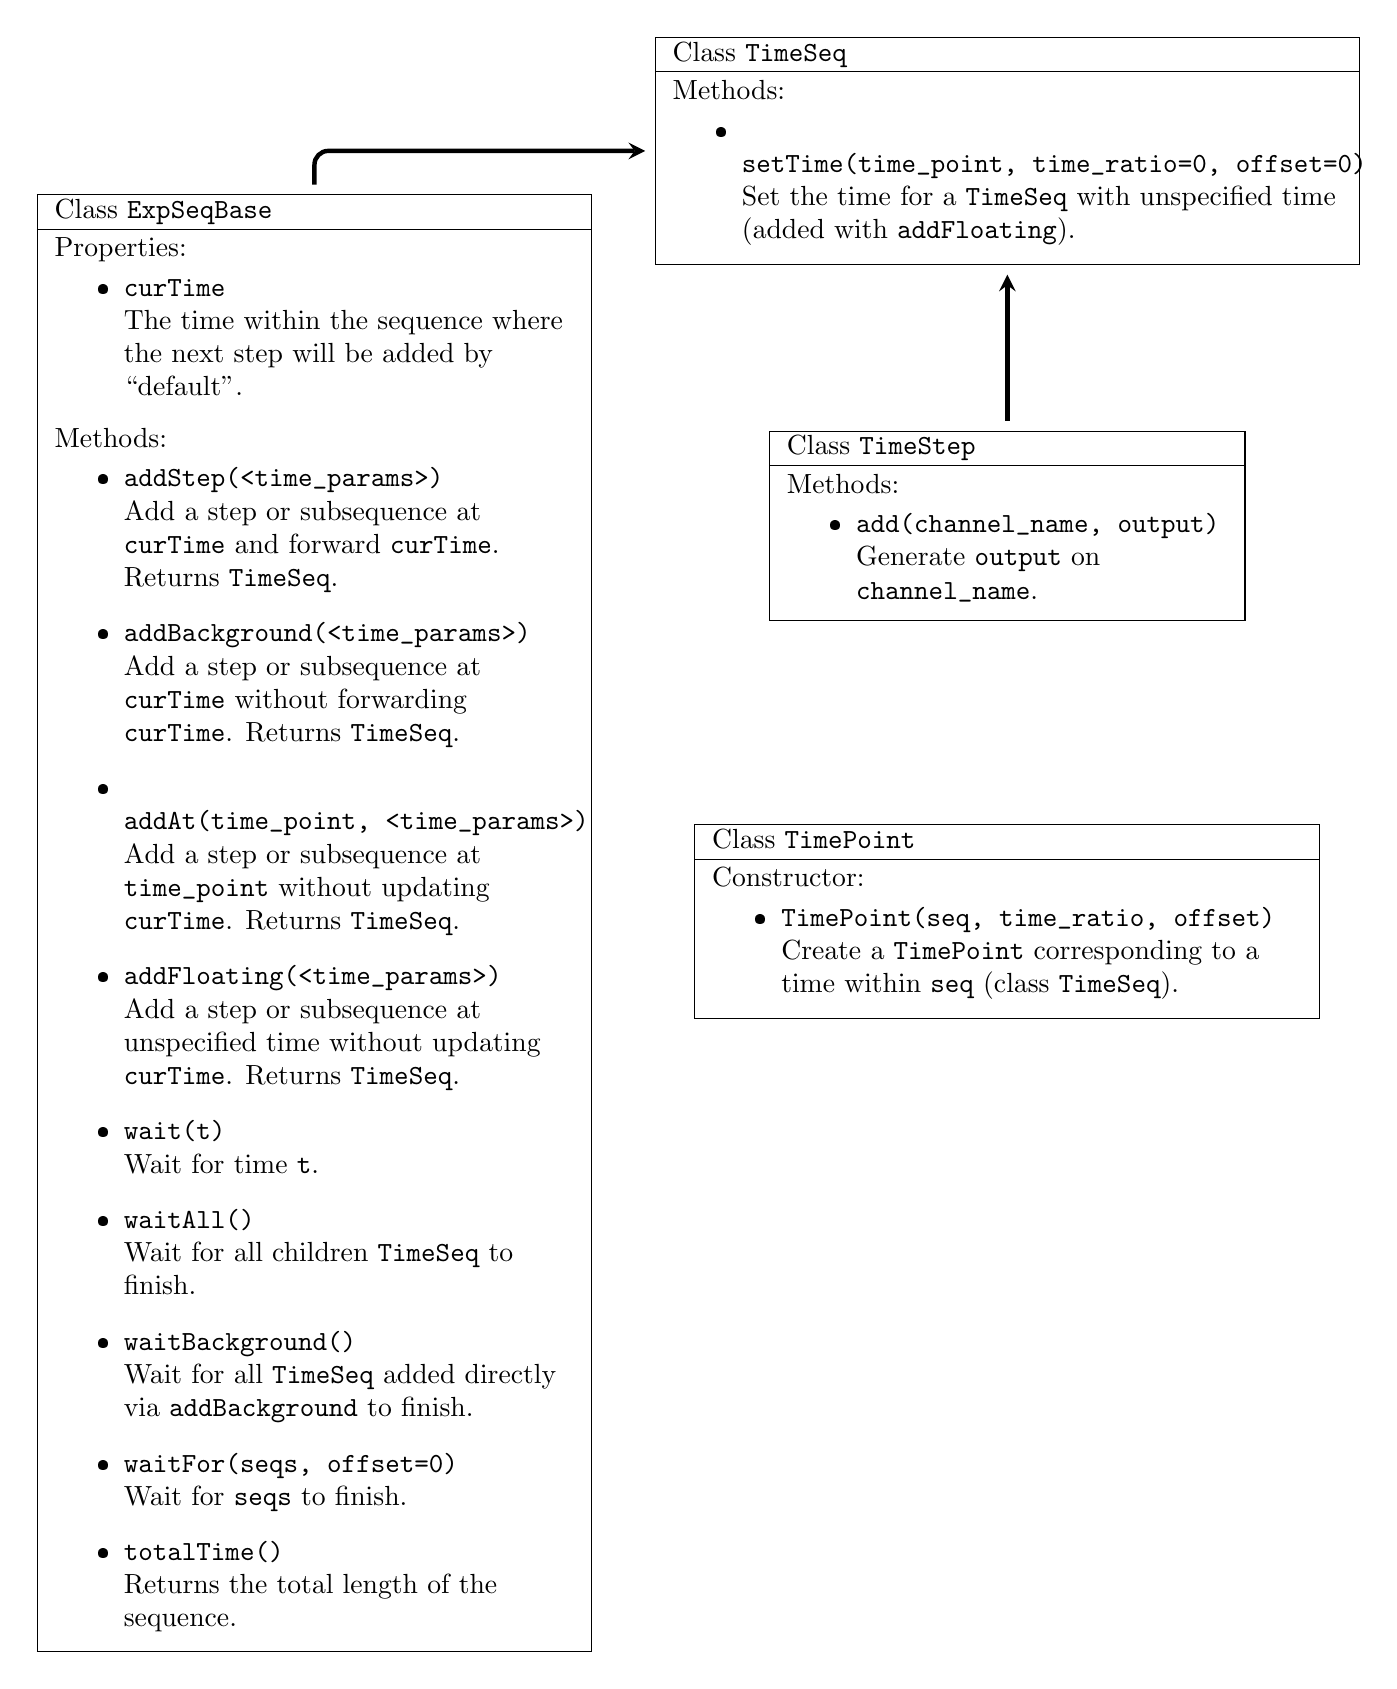
\begin{tikzpicture}
  \node[below] (TimeSeq) at (10, 2) {
    \begin{tabular}{|l|}
      \hline
      Class \verb`TimeSeq`\\\hline
      \begin{minipage}{8.5cm}
        \vspace{0.1cm}
        Methods:\vspace{-0.2cm}
        \raggedright
        \begin{itemize}
        \item \verb`setTime(time_point, time_ratio=0, offset=0)`\\
          Set the time for a \verb`TimeSeq` with unspecified time
          (added with \verb`addFloating`).
        \end{itemize}\vspace{-0.05cm}
      \end{minipage}
      \\\hline
    \end{tabular}
  };
  \node[below] (ExpSeqBase) at (1.2, 0) {
    \begin{tabular}{|l|}
      \hline
      Class \verb`ExpSeqBase`\\\hline
      \begin{minipage}{6.6cm}
        \vspace{0.1cm}
        Properties:\vspace{-0.2cm}
        \raggedright
        \begin{itemize}
        \item \verb`curTime`\\
          The time within the sequence where the next step will be added by ``default''.
        \end{itemize}\vspace{-0.05cm}
        Methods:\vspace{-0.2cm}
        \raggedright
        \begin{itemize}
        \item \verb`addStep(<time_params>)`\\
          Add a step or subsequence at \verb`curTime` and forward \verb`curTime`.
          Returns \verb`TimeSeq`.
        \item \verb`addBackground(<time_params>)`\\
          Add a step or subsequence at \verb`curTime` without forwarding \verb`curTime`.
          Returns \verb`TimeSeq`.
        \item \verb`addAt(time_point, <time_params>)`\\
          Add a step or subsequence at \verb`time_point` without updating \verb`curTime`.
          Returns \verb`TimeSeq`.
        \item \verb`addFloating(<time_params>)`\\
          Add a step or subsequence at unspecified time without updating \verb`curTime`.
          Returns \verb`TimeSeq`.
        \item \verb`wait(t)`\\
          Wait for time \verb`t`.
        \item \verb`waitAll()`\\
          Wait for all children \verb`TimeSeq` to finish.
        \item \verb`waitBackground()`\\
          Wait for all \verb`TimeSeq` added directly via \verb`addBackground` to finish.
        \item \verb`waitFor(seqs, offset=0)`\\
          Wait for \verb`seqs` to finish.
        \item \verb`totalTime()`\\
          Returns the total length of the sequence.
        \end{itemize}\vspace{-0.05cm}
      \end{minipage}
      \\\hline
    \end{tabular}
  };
  \node[below] (TimeStep) at (10, -3) {
    \begin{tabular}{|l|}
      \hline
      Class \verb`TimeStep`\\\hline
      \begin{minipage}{5.6cm}
        \vspace{0.1cm}
        Methods:\vspace{-0.2cm}
        \raggedright
        \begin{itemize}
        \item \verb`add(channel_name, output)`\\
          Generate \verb`output` on \verb`channel_name`.
        \end{itemize}\vspace{-0.05cm}
      \end{minipage}
      \\\hline
    \end{tabular}
  };
  \node[below] at (10, -8) {
    \begin{tabular}{|l|}
      \hline
      Class \verb`TimePoint`\\\hline
      \begin{minipage}{7.5cm}
        \vspace{0.1cm}
        Constructor:\vspace{-0.2cm}
        \raggedright
        \begin{itemize}
        \item \verb`TimePoint(seq, time_ratio, offset)`\\
          Create a \verb`TimePoint` corresponding to a time within \verb`seq`
          (class \verb`TimeSeq`).
        \end{itemize}\vspace{-0.05cm}
      \end{minipage}
      \\\hline
    \end{tabular}
  };
  \draw[->,>=stealth,line width=1.6] (TimeStep.north) -- (TimeSeq.south);
  \draw[->,>=stealth,line width=1.6,rounded corners=5pt] (ExpSeqBase.north) |- (TimeSeq.west);
\end{tikzpicture}

\end{document}
